\section{Computational results}
\label{sec:experimental_design}


This section presents the empirical evaluation of our DD-based cut generation procedures. We first focus on the quality of the generated cuts at the root node, in terms of gap reduction and computational efficiency, and compare with alternatives in the literature. Then, we test the efficiency of our procedures for solving instances from the literature to optimality using a B\&B mechanism with cuts added at the root node, and compare them with existing alternatives. %These analyses enable us to understand the comparative advantages of DD-based valid inequalities with traditional IP strategies.

 
\subsection{Experimental setup}


We consider two datasets commonly used in the literature: LABS and VISION.  The LABS instances are the low-autocorrelation binary sequence instances distributed in POLIP and MINLPLib~\cite{polip,minlplib,delPiaWalter2024simple}. Specifically, we consider instances with fewer than 5000 multilinear terms and discard the \texttt{autocorr\_bern20-03} instance (which solves at the root node), for a total of 22 instances. The VISION benchmark consists of the 45 image-restoration instances introduced in the BPO literature~\cite{delPiaKhajaviradSahinidis2020impact}, with image sizes $10\times 10$, $10\times 15$, and $15\times 15$.

Our experimental comparison considers four families of cut-generation routines (i.e., LT, FS, EX, and PT), all of which are applied at the root node, as follows. LT denotes the literature-support baseline, which separates the violated two-link, flower, and odd $\beta$-cycle inequalities of length 3 found by well-known separators. FS  corresponds to the DD separation on the same fixed supports used by LT to test whether the DD separator can recover comparable or stronger cuts from those supports. EX$M$ denotes DD separation on expanded literature supports, where $M\in \{4,5,6,7,8\}$ is the hyperedge cap in Algorithm~\ref{alg:expanded_support_mode}. Lastly, PT$q$ is the partition-support strategy, where $q\in \{0,1,2,3,4\}$ is the partition size parameter. Specifically, the approach considers $r=\max_{e\in E}|e|$ to be the rank of the instance hypergraph, and each PT$q$ strategy considers a vertex partition generated with target size $r+q$, inducing a section hypergraph as described in  Algorithm~\ref{alg:partition_support_mode}. %The parameter $q$ therefore controls how much larger each generic local support is than a maximum-size hyperedge. We test $q\in \{0,1,2,3,4\}$, and report the corresponding variants as PT0, PT1, PT2, PT3, and PT4. Branch-and-bound experiments use the same families except FS, which was evaluated only at the root.

All DD-based CGLPs use the same interior point $\bomega$.
For each local support hypergraph $G_S=(V_S,E_S)$, we set
$
\omega_v=\frac{1}{2}
$
for each $v\in V_S$ and
$
\omega_e=2^{-|e|}
$
for each $e\in E_S$.

Our methodology is implemented in Python 3.11.15 using Gurobi 13.0.1, with a 3600\,s time limit across all experiments. We use a single-thread (i.e., \texttt{Threads=1}), set \texttt{PreCrush=1} to allow user cuts to be translated through presolve, and deactivate native cuts in Gurobi (i.e., \texttt{Cuts=0}, \texttt{MIPSepCuts=0}, and \texttt{CutPasses=0}) to avoid interference of external cuts in our comparisons. The experiments were run on the \textit{Ingeniería UC Cluster} using SLURM, equipped with an AMD EPYC 9354 processor and 256\,GB of RAM.

A separation round solves the current LP relaxation, searches for local supports under
the selected strategy, and adds at most $\lceil 0.05|E|\rceil$ violated cuts. For
neighborhood-based strategies, the initial neighborhood contains 300 hyperedges and is
expanded by 30 hyperedges whenever no candidate support is found, until the search budget is exhausted.

In all experiments, cuts are added to the root node based on the following criteria. Separation stops when a round finds no cuts; for PT, up to five consecutive no-cut rounds are allowed before stopping. Separation also stops if the average LP improvement per cut over the last 50 rounds is less than $10\%$ of the historical average LP improvement per cut, or if a round time exceeds $2.5$ times the median separation time over the last 20 rounds. In particular, the last stopping criterion is used to avoid adding uninformative cuts, which, in turn, increase computational time and model size.  

\subsection{Root relaxation and facet audit}

We first evaluate the efficiency of the proposed DD-based cuts across different strategies and relative to cuts from the literature. Moreover, we use the facet dimension certificate from Section \ref{sec:dimension_facet_audit} to check the quality of the generated cuts and determine the portion of them that are facet-defining. 

Table~\ref{tab:root-main-final-candidate} reports the root-relaxation performance across all alternatives. Column ``Gap'' is the average root gap left after separation, while ``C\%'' reports the average percentage of the initial root gap closed by the
generated cuts~\cite{delPiaWalter2024simple}: for each instance, if $SR$
is the root objective value before adding our cuts, $DB$ is the root objective value
after separation, and $PRIMAL$ is the reference integer objective value, then
$ \mathrm{C\%} = 100\cdot \frac{DB-SR}{PRIMAL-SR}$.
Column ``Time'' is the mean root-separation time, while ``CM'' measures the average number of cuts generated, and ``C\% / 1000'' reports the mean percentage of gap closed divided by the mean number of cuts in thousands. 


% Root table rebuilt from cleaned final seed1 logs.
\begin{table}[t]
\centering
%\scriptsize
\caption{Root-relaxation performance on tested instances.}
\label{tab:root-main-final-candidate}
%\resizebox{\textwidth}{!}{%
\begin{tabular}{llrrrrr}
\toprule
Dataset & Method & Gap & C\% & Time & CM & C\% / 1000 \\
\midrule
LABS & LT & 437.15 & 60.97 & 47.02 & 3412.4 & 17.87 \\
LABS & FS & 488.16 & 57.63 & 51.61 & 2801.4 & 20.57 \\
LABS & EX4 & 265.42 & 75.58 & 42.10 & 2092.7 & 36.12 \\
LABS & EX5 & 214.52 & 78.65 & 42.56 & 1892.8 & 41.55 \\
LABS & EX6 & 216.52 & 78.49 & 49.09 & 1615.8 & 48.57 \\
LABS & EX7 & 205.16 & 79.28 & 50.30 & 1670.5 & 47.46 \\
LABS & EX8 & 224.29 & 78.06 & 51.01 & 1532.7 & 50.93 \\
LABS & PT0 & 57.09 & 91.31 & 32.22 & 2202.5 & 41.46  \\
LABS & PT1 & 51.97 & 91.82 & 35.25 & 1677.7 & 54.73  \\
LABS & PT2 & 45.37 & 92.33 & 24.65 & 1175.5 & 78.55  \\
LABS & PT3 & 45.46 & 92.36 & 30.67 & 914.4 & 101.01  \\
LABS & PT4 & 43.28 & 92.40 & 28.92 & 686.5 & 134.59  \\
\addlinespace
VISION & LT & 5.86 & 95.82 & 21.25 & 1211.4 & 79.10 \\
VISION & FS & 9.17 & 93.44 & 13.13 & 1021.8 & 91.45 \\
VISION & EX4 & 9.68 & 93.15 & 17.67 & 862.9 & 107.95 \\
VISION & EX5 & 2.06 & 98.53 & 22.41 & 855.3 & 115.21 \\
VISION & EX6 & 0.55 & 99.59 & 16.43 & 548.7 & 181.52 \\
VISION & EX7 & 0.73 & 99.50 & 19.03 & 597.8 & 166.44 \\
VISION & EX8 & 1.69 & 98.83 & 21.00 & 607.3 & 162.74 \\
VISION & PT0 & 0.00 & 100.00 & 5.14 & 675.4 & 148.06 \\
VISION & PT1 & 0.04 & 99.98 & 5.14 & 662.9 & 150.82 \\
VISION & PT2 & 0.02 & 99.99 & 5.28 & 624.6 & 160.07 \\
VISION & PT3 & 0.19 & 99.87 & 5.81 & 662.6 & 150.73 \\
VISION & PT4 & 0.01 & 99.99 & 6.20 & 646.4 & 154.69 \\
\bottomrule
\end{tabular}
%}%
\end{table}


We first note that LT and FS have similar performance in both datasets, which is the intended validation outcome. This result shows that when the DD separator is given the same structural information as the literature separator, it recovers comparable root behavior. The smaller number of cuts in FS is likely due to cut collisions: if two literature structures share part of their support, DD separation may yield the same inequality over the shared region, so fewer distinct cuts are added.

In contrast, we observe significant improvement when using the DDs to represent more complex structures.  On LABS, the PT family dominates: PT4 gives the smallest final root gap, closing $92.40\%$ of the initial gap with only $686.5$ cuts on average, and it also has the largest Gap closed per 1000 cuts value. The EX family also improves substantially over LT: EX4 reduces the final average gap from $437.15$ to $265.42$, and EX7 yields the smallest EX final gap. On VISION, the result is even sharper: PT0 closes $100.00\%$ of the root gap across all tested instances, yielding perfect root relaxation on this benchmark set under our experimental configuration. The EX methods also nearly close the gap, with EX6 reaching $99.59\%$, but PT0 obtains the tightest relaxation with the fastest average separation time. 

We also observed that stronger supports change the nature of the generated cuts. In the EX family, increasing the expansion generally reduces the number of cuts while increasing the gap closed per 1000 cuts. This suggests that richer local DDs produce stronger individual inequalities, leaving fewer violated structures available after each round. The same pattern is even clearer in the PT family on LABS: as the $q$ parameter increases, the method produces fewer cuts but achieves higher efficiency. Thus, the larger local DDs are not merely producing more inequalities; they are producing more informative inequalities. Moreover, we observed that the computation time (i.e., column ``Time'') of all DD-based strategies is similar, reinforcing the practical benefits of DD-based cut generation strategies. 

% Facet table rebuilt from cleaned final seed1 logs.
\begin{table}[b]
\centering
%\scriptsize
\caption{Facet-audit summary on tested instances. }
\label{tab:facet-audit-root-summary}
%\resizebox{\textwidth}{!}{%
\begin{tabular}{llrrrrr}
\toprule
Dataset & Method & Max \% & $I_K$ F\% & $I_K$ R\% & G F\% & GK \% \\
\midrule
LABS & LT & 27.4 & 0.0 & 53.3 & 0.0 & 85.7 \\
LABS & FS & 22.4 & 0.0 & 53.5 & 0.0 & 91.3 \\
LABS & EX4 & 38.3 & 31.6 & 90.9 & 31.6 & 97.5 \\
LABS & EX5 & 67.0 & 64.2 & 92.6 & 64.2 & 98.7 \\
LABS & EX6 & 99.8 & 97.8 & 92.9 & 97.8 & 99.6 \\
LABS & EX7 & 99.8 & 98.3 & 93.0 & 98.3 & 99.2 \\
LABS & EX8 & 99.8 & 98.3 & 93.0 & 98.3 & 99.7 \\
LABS & PT0 & 92.4 & 92.4 & 93.3 & 92.4 & 100.0 \\
LABS & PT1 & 95.0 & 94.9 & 95.0 & 94.9 & 100.0 \\
LABS & PT2 & 96.7 & 96.6 & 96.6 & 96.6 & 100.0 \\
LABS & PT3 & 96.6 & 96.5 & 97.2 & 96.5 & 100.0 \\
LABS & PT4 & 96.8 & 96.6 & 97.7 & 96.6 & 99.9 \\
\addlinespace
VISION & LT & 60.0 & 44.0 & 74.8 & 44.0 & 87.5 \\
VISION & FS & 57.7 & 51.8 & 79.6 & 51.8 & 95.0 \\
VISION & EX4 & 52.4 & 49.1 & 90.2 & 49.1 & 97.3 \\
VISION & EX5 & 78.6 & 52.6 & 79.0 & 52.7 & 78.9 \\
VISION & EX6 & 93.0 & 65.0 & 86.0 & 66.3 & 77.4 \\
VISION & EX7 & 100.0 & 59.5 & 88.1 & 67.2 & 67.5 \\
VISION & EX8 & 100.0 & 60.4 & 88.4 & 68.1 & 68.3 \\
VISION & PT0 & 86.7 & 52.5 & 88.9 & 59.1 & 72.5 \\
VISION & PT1 & 93.0 & 53.1 & 88.5 & 60.6 & 67.9 \\
VISION & PT2 & 95.5 & 57.1 & 88.8 & 64.5 & 69.3 \\
VISION & PT3 & 94.2 & 55.8 & 88.9 & 62.7 & 69.2 \\
VISION & PT4 & 96.2 & 58.8 & 89.3 & 65.8 & 70.0 \\
\bottomrule
\end{tabular}
%}%
\end{table}



To further analyze the quality of the generated cuts, we apply our DD-based dimension certificate procedure (i.e., Algorithms \ref{alg:dd_dimension_audit} and~\ref{alg:ik_certificate_audit}) to all generated cuts and report the results in Table~\ref{tab:facet-audit-root-summary}. Column ``Max \%'' is the percentage of audited cuts whose support is maximal in the selected local hypergraph. Column ``$I_K$ F\%'' is the percentage certified as facet-defining for the local $I_K$ relaxation by Algorithm~\ref{alg:ik_certificate_audit}. Column ``$I_K$ R\%'' measures the average ratio between the certified face dimension and the target local dimension, and ``G F\%'' is a conservative lower bound on the percentage of cuts certified as globally facet-defining. Lastly, ``GK \%'' reports the percentage of audited cuts for which the global status could be resolved within the audit budget. If the $I_K$ test does not certify facetness, a global audit is attempted only when the corresponding global DD can be built and audited within a 60\,s limit; otherwise, the global status is left unresolved. The diagnostic audit time is excluded from the reported algorithmic wall-clock times.


Table~\ref{tab:facet-audit-root-summary}  supports the results reported in Table~\ref{tab:root-main-final-candidate}. On LABS, LT and FS generate many cuts, but essentially none are certified as $I_K$ facets. By contrast, EX6 and larger expansions produce cuts that are almost always maximal and overwhelmingly $I_K$-facet-defining, while the PT variants achieve similarly strong certification rates. On VISION, the audit gives a more nuanced but still positive picture. The strongest expanded supports, especially EX7 and EX8, reach $100.0\%$ maximality and have the largest global-certification lower bounds among the EX methods, but their global status is often unresolved within the conservative 60\,s audit budget. The PT methods have lower local facet rates than on LABS, but still certify a large fraction of cuts and, as Table~\ref{tab:root-main-final-candidate} shows, PT0 closes the root gap completely on the tested VISION instances. Taken together, the root and audit results support the main claim of the paper: DD separation is most useful not as another named family of inequalities, but as a black-box mechanism that can take literature-derived structures, expand the support seen by the separator, and produce stronger inequalities than the original structures alone.


\subsection{B\&B performance}

We next evaluate whether the stronger root relaxations translate into better B\&B performance. To ensure a clean comparison, these experiments consider cuts added at the root node by a cutting-plane procedure; that is, root separation is performed on an explicit LP relaxation before tree search begins. Thus, all found cuts are added to this LP model, and we then run Gurobi's B\&B procedure over its MILP version. %In the PT family, each selected DD is allowed to produce up to three cuts, provided that each cut satisfies the violation tolerance imposed by the implementation.



% BB table rebuilt from cleaned final seed1 logs.
\begin{table}[t]
\centering
%\scriptsize
\caption{Branch-and-bound performance on tested instances.}
\label{tab:bb-main-final-candidate}
%\resizebox{\textwidth}{!}{%
\begin{tabular}{llrrrrr}
\toprule
Dataset & Method & Solved & Time & Nodes & Gap \% & C\% \\
\midrule
LABS & LT & 11 & 711.49 & 1717587 & 106.38 & 60.97 \\
LABS & EX4 & 10 & 466.93 & 1412006 & 60.54 & 75.58 \\
LABS & EX5 & 10 & 548.47 & 1768355 & 58.04 & 78.65 \\
LABS & EX6 & 10 & 575.08 & 1779272 & 49.98 & 78.49 \\
LABS & EX7 & 11 & 687.33 & 1667117 & 54.06 & 79.28 \\
LABS & EX8 & 10 & 520.01 & 1771057 & 52.00 & 78.06 \\
LABS & PT0 & 11 & 170.17 & 150556 & 37.17 & 91.31 \\
LABS & PT1 & 11 & 492.98 & 72437 & 51.48 & 91.82 \\
LABS & PT2 & 11 & 689.01 & 47030 & 69.64 & 92.33 \\
LABS & PT3 & 10 & 496.79 & 79766 & 47.30 & 92.36 \\
LABS & PT4 & 10 & 527.26 & 57131 & 44.09 & 92.40 \\
\addlinespace
VISION & LT & 40 & 71.79 & 96337 & 2.41 & 95.82 \\
VISION & EX4 & 36 & 218.73 & 573610 & 4.61 & 93.15 \\
VISION & EX5 & 45 & 31.16 & 1342 & -- & 98.53 \\
VISION & EX6 & 45 & 17.36 & 2 & -- & 99.59 \\
VISION & EX7 & 45 & 19.99 & 4 & -- & 99.50 \\
VISION & EX8 & 45 & 22.05 & 6 & -- & 98.83 \\
VISION & PT0 & 45 & 5.76 & 1 & -- & 100.00 \\
VISION & PT1 & 45 & 5.89 & 2 & -- & 99.98 \\
VISION & PT2 & 45 & 6.03 & 1 & -- & 99.99 \\
VISION & PT3 & 45 & 7.08 & 1 & -- & 99.87 \\
VISION & PT4 & 45 & 7.35 & 1 & -- & 99.99 \\
\bottomrule
\end{tabular}
%}%
\end{table}


Table~\ref{tab:bb-main-final-candidate} reports B\&B performance of all procedures except FS, which was evaluated only at the root node as a validation benchmark. In the table, column ``Solved'' gives the number of instances solved within the 3600\,s limit. Column ``Time'' corresponds to the average solve time computed only over solved runs, ``Nodes'' reports the mean number of B\&B nodes, and ``Gap \%'' is the mean final gap percent computed only over instances that hit the time limit. The last column repeats the root gap closed (i.e.,  ``C\%''), allowing us to compare root strength against downstream tree-search behavior.

On LABS instances, PT0 is the strongest practical B\&B setting in terms of instances solved, time, and gap. This is notable because PT0 is not the strongest PT configuration at the root. The result suggests that the cuts that close the most root gap are not necessarily the cuts that produce the best B\&B behavior. In particular, this result can be explained by the fact that PT0 yields significantly more cuts than the other PT strategies (see Table \ref{tab:root-main-final-candidate}), which, in turn, can help the B\&B algorithm prove optimality. Nonetheless, we note that all PT strategies perform quite well when compared to the EX strategies and the LT baseline.

On VISION, the result obtained at the root node essentially carries over to B\&B. PT strategies solve all 45 instances at the root node and yield the fastest solve times. This is consistent with the root table, where PT0 closes $100.00\%$ of the root gap on VISION, and the other alternatives more than $99.8\%$. The EX methods also perform strongly once the expansion is large enough: EX5--EX8 solve all instances, and EX6 is the fastest expanded-support method. Overall, the B\&B results reinforce the main computational message: DD support expansion improves performance, but the best strategy is not necessarily the one that maximizes root closure.

\begin{figure}[t]
    \centering
    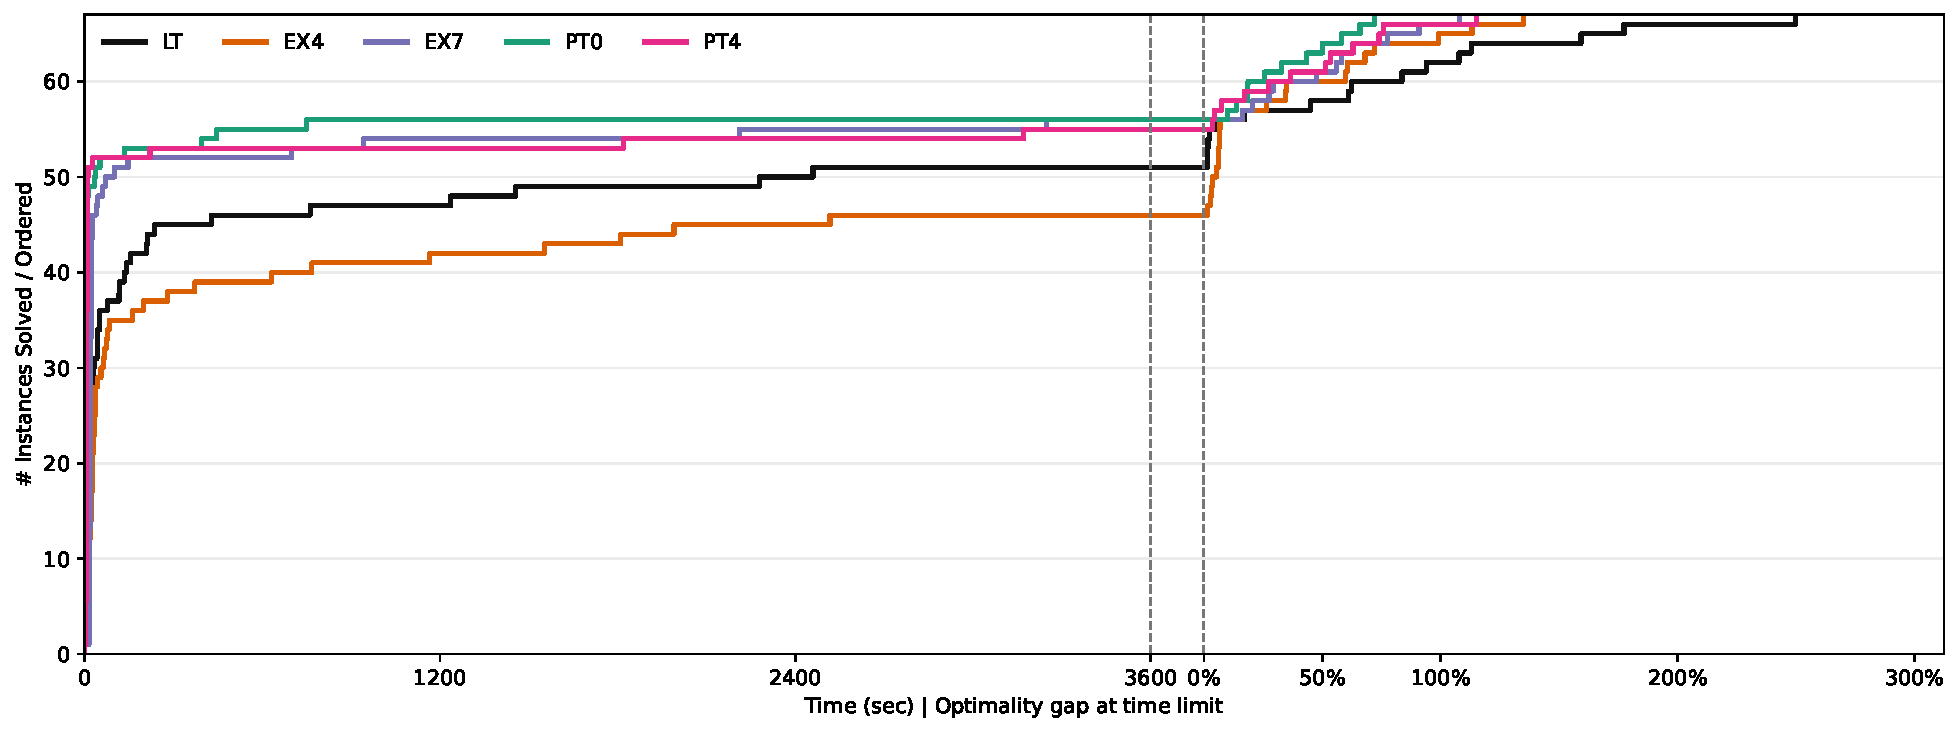
\includegraphics[width=0.96\textwidth]{Figures/results/bb_profile_final_truth_cp0_champion_modes.pdf}
    \caption{B\&B profile for representative methods.}
    \label{fig:bb-profile-final}
\end{figure}

Figure~\ref{fig:bb-profile-final} summarizes the same behavior across the two datasets. The plot depicts only two strategies per family (i.e., EX4, EX7, PT0, PT4) to avoid overcrowding. The left part of the plot shows the cumulative number of solved instances over time, while the right part is a cumulative gap plot for the instances that reach the time limit. Once again, we see that the PT strategies and the larger EX excel in both runtime and optimality gap compared to our baseline LT. Also, it is interesting to see that EX4 has poor performance, which is mostly explained by the fact that the underlying DDs do not represent structures as rich as those of the other alternatives, thus, providing weaker cuts as shown in Tables \ref{tab:root-main-final-candidate} and \ref{tab:facet-audit-root-summary}.

\subsection{Discussion}

These results show that the main gains from our procedures stem from strengthening the support prior to separation. Expanded supports improve substantially over the fixed-support baseline as $M$ increases, and the partition supports are the strongest family overall. On LABS, the PT family yields the best root gaps and the best B\&B behavior among the tested DD-based strategies; in particular, PT0 achieves the fastest solved-instance time and the smallest remaining gap among the unsolved instances, while deeper partition levels close slightly more of the root gap but do not translate into better B\&B performance. On VISION, the same pattern is even sharper: PT0 closes the full root gap on all tested instances and gives the fastest solve times. On VISION, EX6 is the strongest configuration among the EX variants, but the partition supports dominate the overall operational comparison.

In a nutshell, DDs provide a mechanism for turning a chosen support into a separation oracle. When that support is the classical literature structure, the method validates itself by producing cuts of comparable strength. When the support is expanded or repartitioned, the same mechanism can generate stronger cuts than the original structure alone could. This supports the interpretation of DDs as a black-box strengthening device: rather than deriving a new family of inequalities by hand for every enlarged structure, we specify the structure and let the DD-based target-cut model separate over it.